
\section{Cas d'utilisation : Dissémination de messages}
\label{net:sec:usecase}

La diffusion de messages d'un nœud à tous les autres est une fonctionnalité
courante des réseaux (\emph{broadcast}). La propagation épidémique
(\emph{gossip})~\cite{birman1999bimodal} constitue un moyen efficace de la
mettre en place. Sa dénomination provient de son fonctionnement : un nœud
choisit un sous-ensemble des membres du réseau et les ``contamine'' en leur
envoyant le message; les nœuds ``infectés'' en font de même; un nœud ayant déjà
envoyé le message ne le renvoie pas. Plus la taille du sous-ensemble choisi est
élevée, plus la probabilité selon laquelle le message parvient à tous les
membres du réseau
augmente~\cite{erdos1959random}. 

\begin{algorithm}
  
\small
\algrenewcommand{\algorithmiccomment}[1]{\hskip2em$\rhd$ #1}

\newcommand{\comment}[1]{\hfill $\rhd$ #1}

\newcommand{\LINEFOR}[2]{%
  \algorithmicfor\ {#1}\ \algorithmicdo\ {#2} %
  }

\newcommand{\LINEIFTHEN}[2]{%
  \algorithmicif\ {#1}\ \algorithmicthen\ {#2} %
  }

\newcommand{\INDSTATE}[1][1]{\State\hspace{\algorithmicindent}}

\begin{algorithmic}[1]
  \Function{broadcast}{$m$} \comment{$m$: \emph{message to send}}
  \State \textbf{let} $chosen \leftarrow getPeers(P,\, \DARKBLUE{fanout})$;
  \For{(\DARKBLUE{$n \in chosen$})}
  \State \textsc{sendTo}($n$, 'broadcast', $m$);
  \EndFor
  \EndFunction

  \Statex

  \Function{onBroadcast}{$m$} \comment{$m$: \emph{received message}}
  \If {($\DARKBLUE{\neg\textsc{alreadyReceived}(m)}$)}
  \State \textsc{broadcast}($m$);
  \EndIf
  \EndFunction
\end{algorithmic}

  \caption[Algorithme de dissémination de
  messages]{\label{net:algo:broadcast}Algorithme de dissémination de messages.}
\end{algorithm}


L'algorithme~\ref{net:algo:broadcast} montre les quelques instructions composant
la dissémination épidémique de messages. L'épanouissement (\emph{fanout})
désigne le nombre de voisins auxquels le message va être envoyé. La fonction
\textsc{getPeers} renvoie autant de nœuds distincts. Dans le cadre d'approches
fournissant une vue partielle de taille constante, cette variable
d'épanouissement est elle aussi constante, et configurée à l'avance. Pour que
les chemins employés lors de la dissémination soient eux aussi aléatoires malgré
la fréquence beaucoup plus faible des échanges du protocole d'échantillonnage,
la taille de la vue est nettement surestimée~\cite{frey2009heterogeneous}. Par
exemple, une vue partielle contient 30 arcs, mais seulement 6 sont employés à
chaque dissémination. Dans le cadre de \SPRAY, nous augmentons les tailles des
vues partielles fournies : lors de l'entrée dans le réseau, un nœud n'ajoute
plus qu'une seule référence au contact mais $c$ doublons; les vues partielles
tendent vers $c.\ln(|\mathcal{N}|)$~\cite{ganesh2003peer}; un nœud détectant un
départ ou une panne ajuste la probabilité de supprimer un arc à
$c \div (|P|+occ)$. La variable d'épanouissement est configurée comme étant une
fraction de la vue partielle. Ainsi l'épanouissement peut s'ajuster
automatiquement pour suivre une progression logarithmique :
$\ln(|\mathcal{N}|)+x$, où $x$ est un entier positif.

La suite met en évidence l'avantage apporté par une variable d'épanouissement
s'ajustant à la taille du réseau. En particulier, nous mesurerons le taux de
réception totale des messages par les membres du réseau. Si au moins un membre
ne reçoit pas le message, alors la réception totale à échouée. Le taux mesuré
est le nombre de messages ayant été reçus par tout les membres sur le nombre de
messages ayant été envoyés.

\begin{figure}
  \begin{center}
    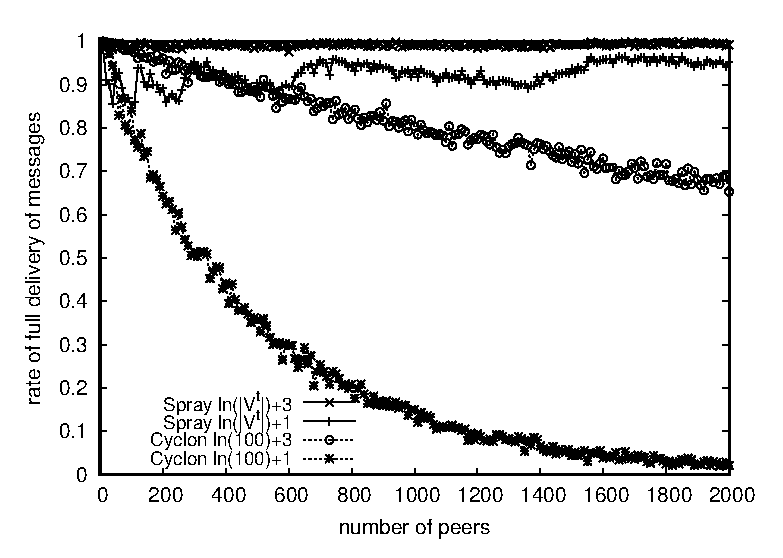
\includegraphics[width=.8\textwidth]{img/spray/hardrate.eps}
    \caption[Hard Rate]{\label{net:fig:hardrate} Hard Rate.}
  \end{center}
\end{figure}


\paragraph{Objectif :} Montrer les bénéfices apportées au mécanisme de
dissémination par un protocole adaptatif d'échantillonnage.
\paragraph{Description :} L'application considérée cible approximativement 100
nœuds. Les vues partielles fournies par \CYCLON sont configurées pour contenir
30 voisins ($6.\ln(100) \approx 6.5 = 30$). Nous considérons 2 configurations
pour l'épanouissement : $\ln(100)+1 \approx 6$ et $\ln(100)+3 \approx 8$. Ces
configurations garantissent une forte probabilité de réception des messages
lorsque le réseau contient 100 nœuds ou moins. De même, nous configurons \SPRAY
pour qu'il fournisse des vues partielles 6 fois plus peuplés qu'à la normale. La
variable d'épanouissement est configurée pour choisir 1 sixième de la vue, soit
$\ln(|\mathcal{N}|)+1$ et $\ln(|\mathcal{N}|)+3$.  Les deux protocoles
d'échantillonnage aléatoire possèdent donc les même configurations pour un
réseau de 100 nœuds. La taille des réseaux considérés grandit de 100 à 2000
nœuds. Nous mesurons à chaque cycle la fraction, sur 1k messages, parvenant à
l'intégralité des membres du réseau.
\paragraph{Résultat :} La figure~\ref{net:fig:hardrate} présente les résultats
de cette simulation. Tout d'abord, nous observons que le taux de réception des
messages.
\paragraph{Explication :}

\begin{figure}
  \begin{center}
    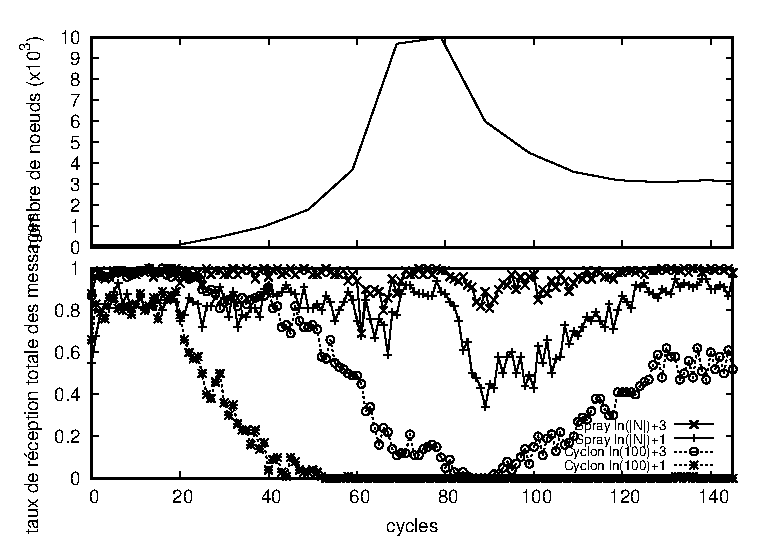
\includegraphics[width=.8\textwidth]{img/spray/peak.eps}
    \caption[Peak]{\label{net:fig:peak} Peak.}
  \end{center}
\end{figure}

\paragraph{Objectif :}
\paragraph{Description :}
\paragraph{Résultat :}
\paragraph{Explication :}

%%% Local Variables:
%%% mode: latex
%%% TeX-master: "../../paper"
%%% End:
